\section{Design Considerations}

\subsection{Reducing Frontal Area and improving the coefficient of drag}

A typical passenger car offer five seats, while the average occupancy rate for private car remains well below two persons per car \cite{ceu_move_study_2022}.

The most aerodynamically efficient way to transport a human would be in a reclined position with their legs aligned with the direction of travel. However, this poses significant challenges in terms of user acceptance and visibility. While vision could be restored through external imaging systems, the disconnect between visual input and physical sensation could lead to motion sickness. A more pragmatic approach to reducing frontal area is to design a smaller, narrower vehicle with one or two seats arranged in a tandem configuration. This layout minimizes width while enabling a more elongated, teardrop-shaped body, which improves aerodynamic efficiency. Additionally, tilting the seats can lower the vehicle’s effective height, further reducing frontal area and drag.


\begin{figure}[h!]
    \centering
    \subfloat{
        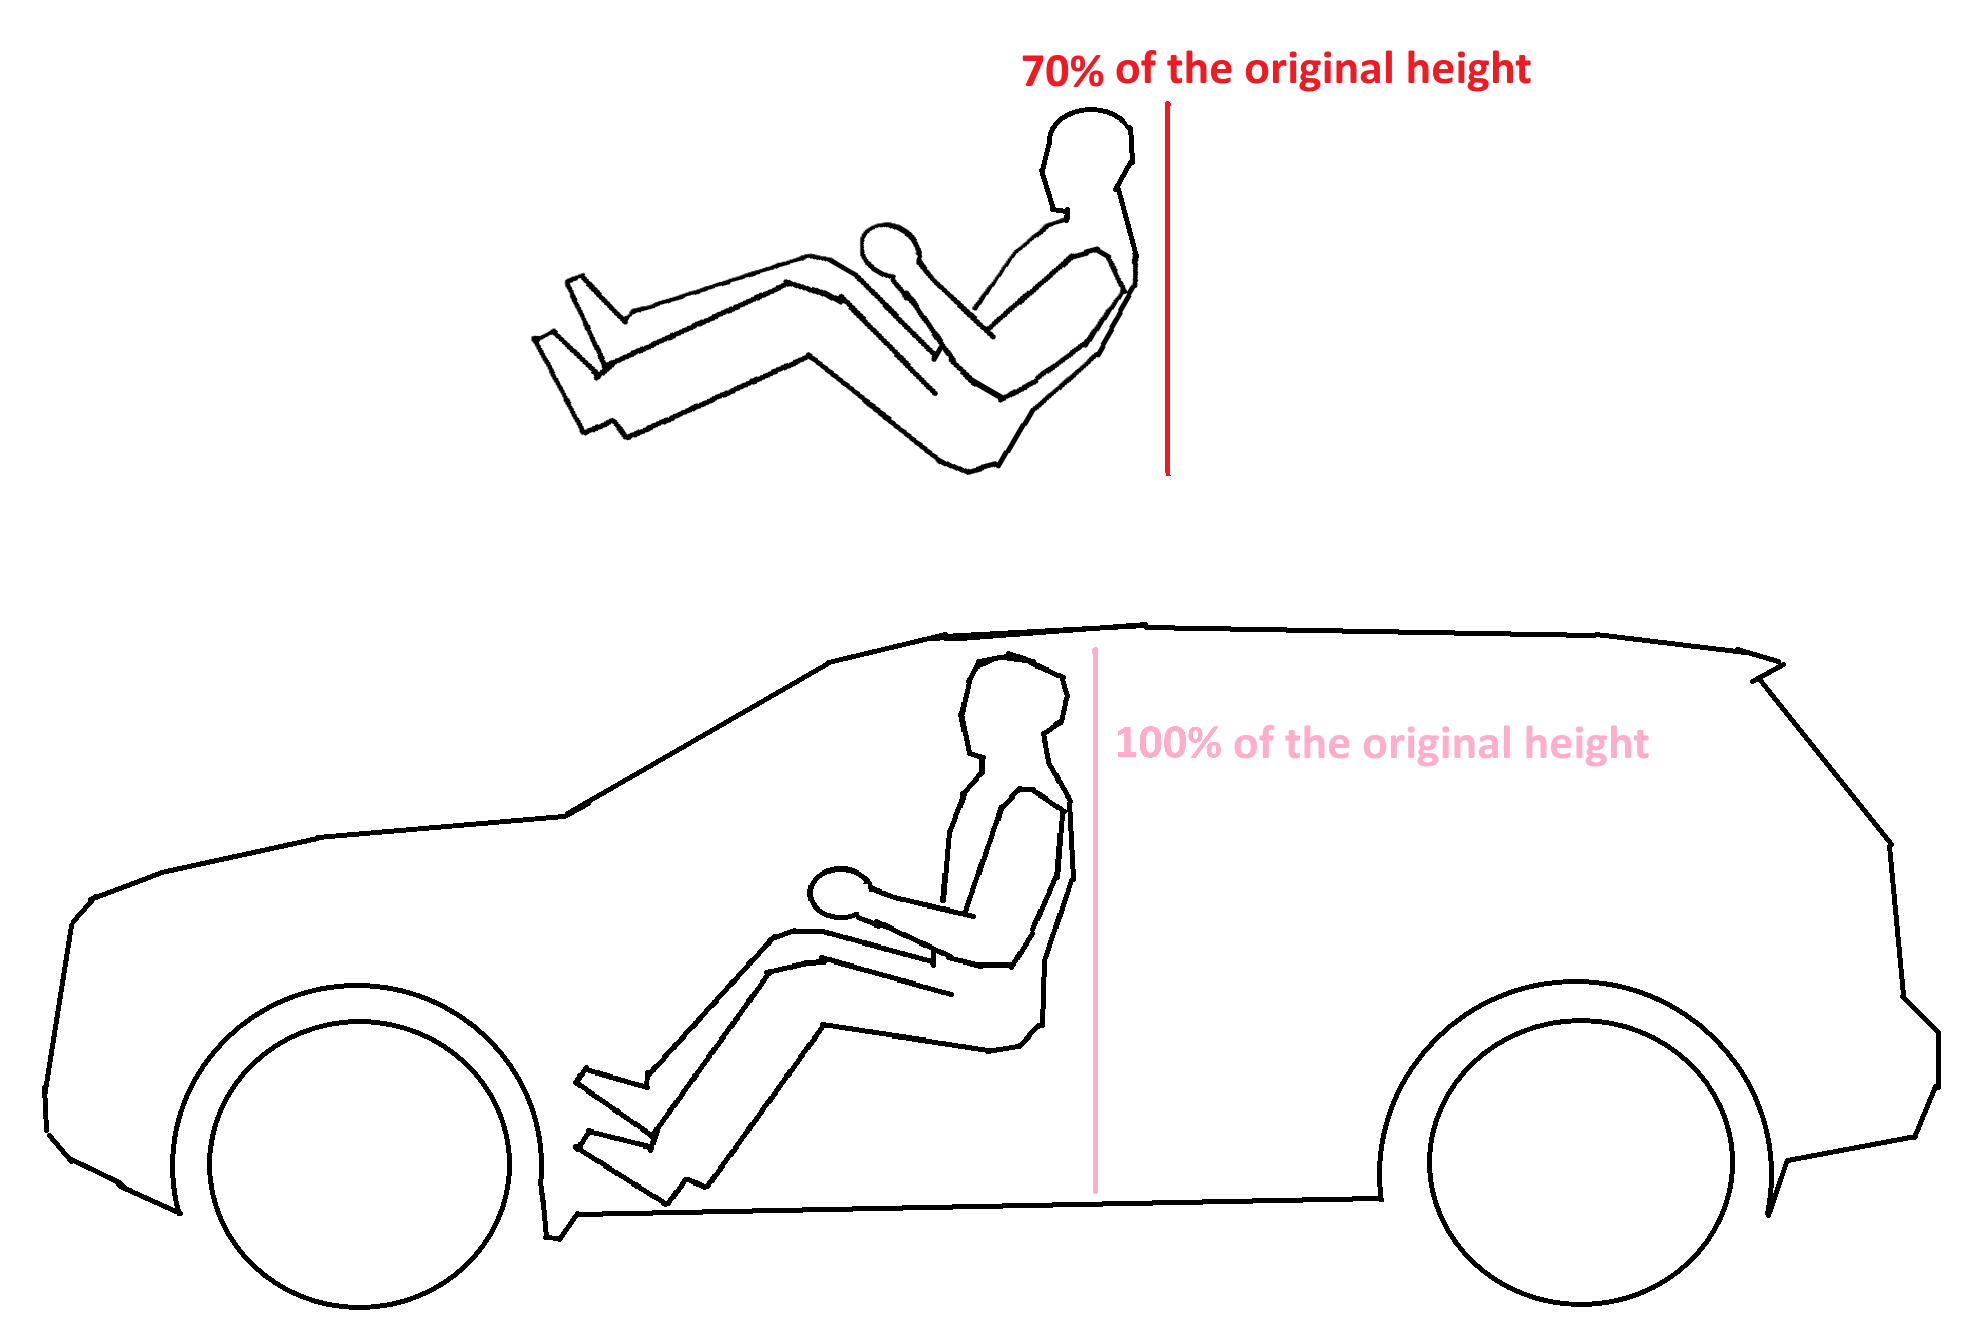
\includegraphics[width=0.47\linewidth]{Figures/ch3_seatingOptimisation.png}
    }
    \hfill
    \subfloat{
        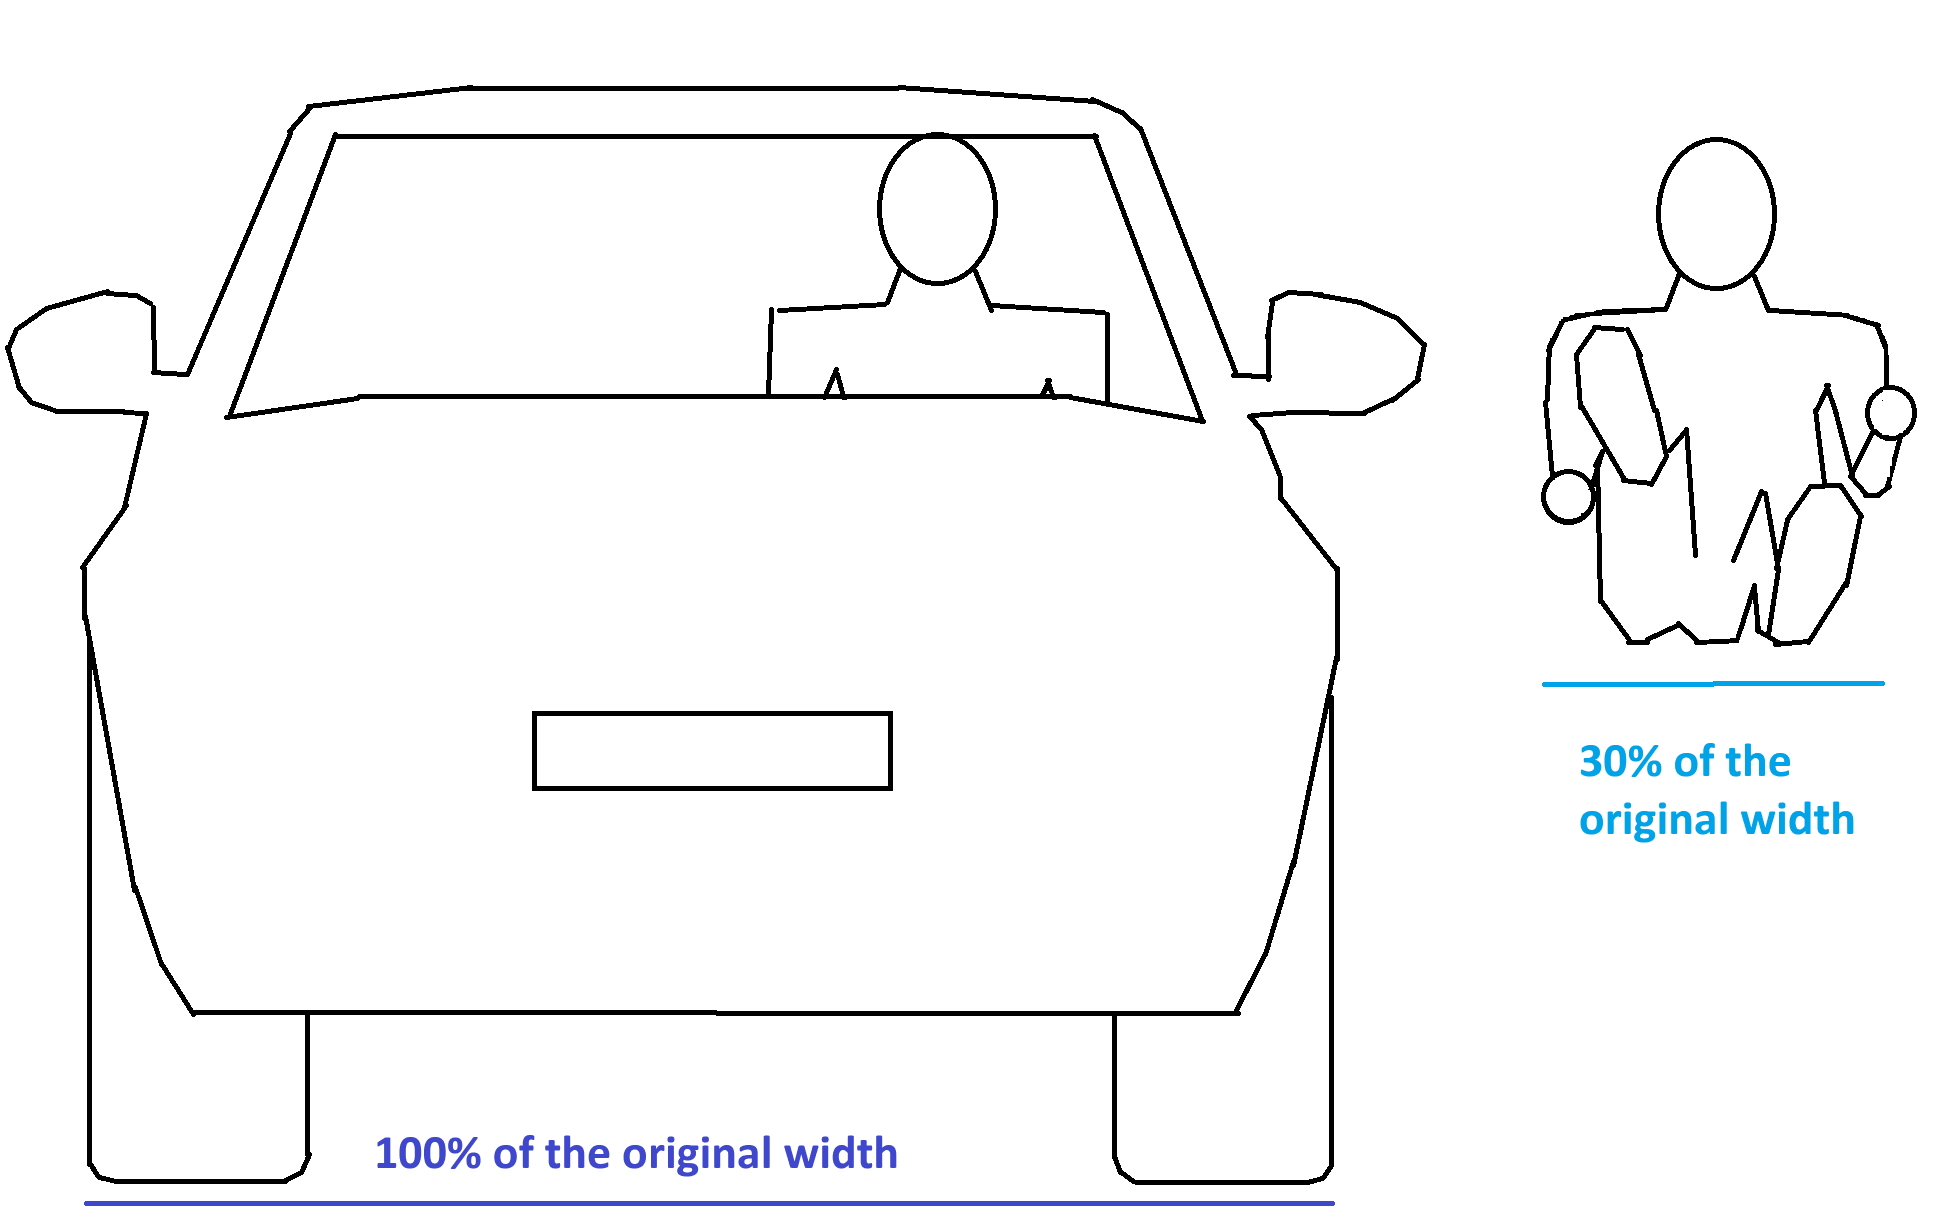
\includegraphics[width=0.47\linewidth]{Figures/ch3_seatingOptimisationFront.png}
    }
    \caption{effect on the frontal area by reclining the seat by 30° and placing passengers one behind another}
    \label{fig:FrontaAreaGraphicsComparison}
\end{figure}

This introduces many challenges.
The first one being the stability of the system. Traditional car are wide and have a low center of mass. This configuration would yield a vehicle which would fall in the category of narrow track vehicle.This category of vehicle share the need to lean during a turn similarly to a bike to prevent tilting over. The second challenge come from entering and exiting the vehicle. To address the exit problem, we could design the leaning system to also allow setting the seat to a position that is easier to exit. The reward for these added complication is the drastic reduction in frontal area.

\subsection{Reducing mass and embodied energy}

The weight of a typical passenger car is largely influenced by safety requirements, comfort expectations, and the perceived need to accommodate multiple passengers. Modern vehicles are equipped with a variety of heavy components, including reinforced steel structures, crash absorption elements, large batteries (for electric vehicles), and extensive infotainment systems. While these features contribute to comfort and safety, they also significantly increase mass and, consequently, energy consumption.

Reducing vehicle mass directly lowers the energy required for acceleration, climbing, braking, and overcoming rolling resistance, leading to improved efficiency. One approach to mass reduction is the use of lightweight materials such as aluminum or composites. However, the choice of material must consider not only its weight but also its embodied energy. For example, while carbon fiber composites offer significant weight savings, their production is highly energy-intensive, and they exhibit poor recyclability, limiting their sustainability benefits.

A more sustainable alternative may be found in natural materials such as wood or bio-based composites. Wood structures, for instance, offer excellent strength-to-weight ratios while requiring significantly less energy to produce than metals or advanced composites. Similarly, PET sheets could provide lightweight, low-cost paneling solutions that reduce both vehicle weight and environmental impact.

Another crucial factor influencing vehicle weight is crash safety. Current safety standards are designed around high-speed impacts, requiring vehicles to be built with reinforced crash structures that increase their mass. However, if we reconsider mobility at lower speeds, the need for such heavy crash protection could be reduced. A vehicle designed for urban environments with a lower top speed would face less severe crash scenarios, allowing for a lighter construction without compromising safety. Instead of heavy reinforcement, safety could be ensured through crumple zones optimized for lower-speed impacts, active safety systems, and improved collision avoidance technologies.

In the end, it's all about finding the right balance between structural integrity, safety, and sustainability. A lighter vehicle, designed with carefully chosen materials and adapted safety considerations, can not only improve efficiency but also significantly reduce its overall carbon footprint of personal mobility.

\subsection{Addressing Visibility and Safety Concerns in Traffic}

When we minimize frontal area, we tend toward low design that are assimilable to velomobile and trike. We will thus look at why such vehicle is not more common and learn from their limitations.

Despite their aerodynamic and energy efficiency advantages, trikes and velomobile remain a niche mode of transportation rather than a mainstream alternative to conventional cars. Several factors contribute to their limited adoption, including economic considerations, perceived safety concerns, and practical usability issues.

One of the main, if not the main challenge, is likely economic in nature. New velomobile often cost north of 10'000 CHF while a brand-new car start at 15'000 CHF. This price difference, hard to justify to a consumer, can be easily explained by the scale economy from cars manufacturer. 

Another challenge is the visibility in traffic. Velomobiles and trikes are lower on the road than conventional cars, making them less noticeable to other road users. While simple solution exist like flags to show their presence, they don't do much to alleviate the feeling of vulnerability of the driver. \cite{velomobile_safety}

Another major barrier to widespread adoption is accessibility, particularly for the elderly and those with mobility impairments. Velomobiles require users to step down into the vehicle and wiggle into a reclined position, which can be difficult for individuals with limited flexibility or strength. Exiting the vehicle can be just as challenging, especially in tight parking spaces or when carrying groceries and other loads.

To address these concerns, one potential solution is to raise the vehicle’s seat and thus center of mass. Improving both the driver’s visibility to other road users and accessibility at the expense of dynamic stability, which will then require a compensation mechanism.


TODO : find a backing source
\newpage

\subsection{Narrow Track and Low Vehicle Geometry (literature review)}
Acknowledge existing solution

Recent development in automotive engineering, more effort recently. multiple geometry, multiple control scheme, which one is better ?

(show the kinematic studied already ( 3 wheel scooter, 4 wheel, diamond, etc) (see connected papers)